\section{Our Approach} \label{sec:fm}

In this section we describe our proposed function merging technique and show
how it merges the motivating examples. Our technique works on any two
arbitrary functions, even when they have few similarities and merging them would
be counter-productive. For that reason, we also introduce a cost model to decide
when it is beneficial to merge two functions (see Section~\ref{sec:profit-model}).
To avoid an expensive quadratic exploration, we integrate our profitability analysis
with an efficient ranking mechanism based on a lightweight fingerprint of the functions.

%% I don't think the compilation pipeline should be here.
%% The optimization does not need to be performed during link-time.
%% I think it is part of our experimental setup, that's way it was in the result section.
%% It could be performed per compilation-unit as well.
%\begin{figure}[t!]
%  \centering
%  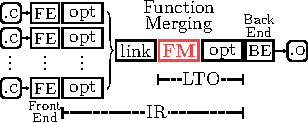
\includegraphics[width=0.7\linewidth]{figs/opt-pipeline.pdf}
%  \caption{The compilation pipeline of our approach.}
%  \label{fig:opt-pipeline}
%\end{figure}

%\subsection{The Compilation Pipeline}
%Our approach is implemented as an LLVM pass to perform at the LLVM IR level. Therefore, it can perform function merging across application
%and library code.

%Figure~\ref{fig:opt-pipeline} shows an overview of the compilation pipeline using our function merging (FM) approach. First, we apply early
%code-size optimizations per compilation-unit (e.g., \update{functions and basic blocks}). Then, function merging and further code-size
%optimizations are applied during monolithic link-time optimization~(LTO). With LTO, object file generation is delayed until all input
%modules are known, instead of being generated per
%compilation-unit, which enables more powerful optimizations based on whole-program analyses. %The baseline uses exactly the same compilation
%%%%pipeline, except for not having any function-merging optimization.

%\subsection{Overview of Our Approach}
\subsection{Overview}
Intuitively, when we are manually merging two functions, in a textual format, we try to visualize them side by side, identifying the
equivalent segments of code and the non-equivalent ones. Then, we use this understanding to create the merged function. In this paper, we
propose a technique that follows this simple yet effective principle. At the core of our technique lies a sequence alignment algorithm,
which is responsible for arranging the code in segments that are either equivalent or non-equivalent.
We implement this technique at the level of the intermediate representation (IR).

\begin{figure}[t!]
  \centering
  %\vspace{-1ex}
  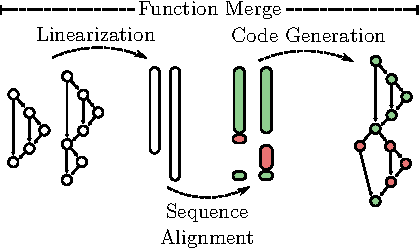
\includegraphics[width=0.85\linewidth]{figs/func-merge-overview.pdf}
  \caption{Overview of our function-merging technique.
           Equivalent segments of code is represented in light green and the non-equivalent ones in dark red.}
           %\fixme{ZW: We need to change the colors and don't use color codes in the text, because the paper may be printed in black and white.}
           %\fixme{Rodrigo: I think it is very ugly to use dashed background, or using other ugly patterns to differenciate things.
           %        I think it is important for the paper to look nice and give a good first impression to the reader.}
		   %\fixme{PP: I don't like patterns either, but the two colours looked the same in b&w or to colourblind people. Made the green light and the red dark to make them distinct.}
           %%By the way, the seq. alignment has a visual structural difference between code that will be merged (blocks in the centre in Fig. 5, and blocks in both functions in this figure.}
           %%compared to code that will not be merged, only one of the functions have a block of code.

  \label{fig:func-merge-overview}
  %\vspace{-1ex}
\end{figure}

The proposed technique consists of three major steps, as depicted in
Figure~\ref{fig:func-merge-overview}.
First, we linearize each function, representing the CFG as a sequence of
labels and instructions.
The second step consists in applying a sequence alignment algorithm, borrowed
from bioinformatics, which identifies regions of similarity between sequences.
The sequence alignment algorithm allows us to arrange two linearized functions
into segments that are equivalent between the two functions and segments where
they differ from one another.
The final step performs the code generation, actually merging the two functions.
Aligned segments with equivalent code are merged, avoiding redundancy, %redundant code,
while the remaining segments where the two functions differ have their code guarded by a function identifier.

At this point, we create a merged list of parameters, including the extra function identifier if there are any
dissimilar segments. 
Arguments of the same type are shared between the functions, without necessarily keeping their original
order.
We also allow for the return types to be different, in which case we use an aggregate type to return values of both types.
If one of them is void, then we do not create an aggregate type, we just return the non-void type.
Given the appropriate function identifier, the merged function is semantically equivalent to the original functions,
so we replace all of their invocations with the new function.
It should be noted that in the special case where we merge identical functions, the output is also identical, emulating
the behavior of function merging in production compilers.

After producing the merged function, the body of the original functions are
replaced by a single call to this new function.
The original functions can sometimes also be completely deleted and all their
calls are replaced to a call to the merged function.
Some of the facts that prohibit the complete removal of the original functions
are the existance of indirect calls to them or when they are available for
external linkage.
 
\subsection{Linearization}

\begin{figure}[t!]
  \centering
  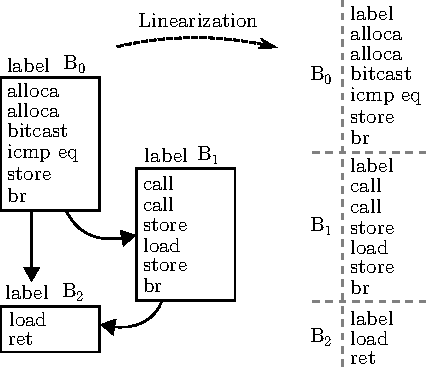
\includegraphics[width=0.7\linewidth]{figs/linearization-example.pdf}
  \caption{Linearizing the CFG of an example function.}
  \label{fig:linearization-example}
\end{figure}

Linearization\footnote{Although linearization of CFGs
usually refers to a predicated representation, % resulting from an if-conversion,
in this paper, we use a simpler definition.} is a key step for enabling the use of sequence alignment. It takes the CFG of the function,
specifies a traversal order of the basic blocks, and for each block outputs its label and its instructions. Linearization
maintains the original ordering of the instructions inside each basic block.
Figure~\ref{fig:linearization-example} shows a simplified example of linearizing the CFG of a
real function extracted from the SPEC CPU2006 \texttt{400.perlbench} benchmark.

%Although this operation is trivial, the specific ordering of the basic blocks
%chosen can have an impact on the merging operation.

%For the linearization, we assume that every basic block has an entry label and
%a terminator instruction which refers explicitly to the successor basic blocks,
%if there are successors.
%This is true for most IRs, such as the LLVM IR, or can be easily adapted.

The traversal order we use for linearization has no effect on the correctness of the transformation
but it can impact its effectiveness. We empirically chose a reverse post-order traversal with a
canonical ordering of successor basic blocks.
%It is also common practice for compilers to rely on prior canonicalizations~\cite{briggs94,liu96}.
This strategy leads to good performance in our experiments.

%a strategy by first ordering the basic blocks in reverse post-order, and then ordering the
%successors in canonical order~\cite{briggs94,liu96}. 
%, e.g., \textit{true} branches before \textit{false} ones.
%Figure~\ref{fig:branch-linearization} shows an example of the linearization
%using the canonical RPO.
%The RPO guarantees that the linearization starts with the entry basic block and then proceeds favoring definitions before uses, except in the presence of loops.
%Although the specifc ordering produced by the canonical linearization may not be optimal,
%in general it shows good results, as it is also common practice for compilers to rely on prior canonicalizations, e.g., canonical loops, canonical induction variables, canonical reassociation, etc.~\cite{briggs94,liu96}.
%By contrast, if, instead, we use an RPO linearization with a uniformly randomized ordering of the successor basic
%blocks, the final code-size reduction of the function-merging optimization can deteriorate by 10\% for individual benchmarks.
%Note that our decision for using the canonical RPO is purely pragmatic and other orderings of the basic blocks could also be used, as long as it produces a sequence of labels followed by instructions.

%\begin{figure}[h]
%  \centering
%  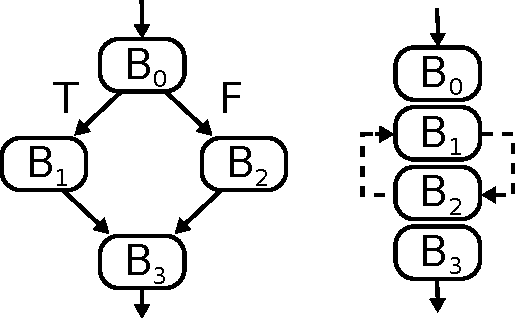
\includegraphics[width=0.6\linewidth]{figs/branch-linearization.pdf}
%  \caption{Linearization using a canonical reverse post-order.
%           The dashed arrows show where a randomized ordering could change the
%           linearization.}
%  \label{fig:branch-linearization}
%\end{figure}

\subsection{Sequence Alignment}

When merging two functions, the goal is to identify which segments of the code are equivalent (and therefore can be merged) and which ones are different.
To avoid breaking the semantics of the original program, we also need to maintain the order of the instructions for each one of the functions.

%%definition of "reduce": present a problem or subject in a simplified form.
After linearization, we reduce the problem of merging functions to the problem of \textit{sequence alignment}. Sequence alignment is an important technique to many areas of science, most notably in molecular biology~\cite{needleman70,smith81,carrillo88,wang94} where, for
example, it is used for identifying homologous subsequences of amino acid in proteins.
Figure~\ref{fig:opcode-align} shows an example of
the sequence alignment between two linearized functions extracted from the \texttt{400.perlbench} benchmark, including the one used in
Figure~\ref{fig:linearization-example}.
Essentially, sequence alignment algorithms insert blank characters in both input sequences in a way that
the final sequences end up having the same size, where equivalent segments are aligned with their matching segments from the other sequence
and non-equivalent segments are paired with blank characters.

Formally, sequence alignment can be defined as follows:
For a given alphabet $\alpha$, a sequence $S$ of $k$ characters is an element of
$\alpha^k$, i.e., $S = (a_1, \ldots a_k)$.
Let $S_1, \ldots, S_m$ be a set of sequences, possibly of different lengths but
all derived from the same alphabet $\alpha$, where
$S_i = (a_1^{(i)}, \ldots, a_{k_1}^{(i)})$, for all $i\in\{1,\ldots,m\}$.
%\begin{equation*}
%\begin{align*}
%S_1 = (a_1^{(1)}, \ldots, a_{k_1}^{(1)})\\
%\dots\\
%S_m = (a_1^{(m)}, \ldots, a_{k_m}^{(m)})
%\end{align*}
%\end{equation*}
Consider an extended alphabet that includes the \textit{blank} character ``$-$'',
i.e., $\beta = \alpha \cup \{-\}$.
An alignment of the $m$ sequences, $S_1, \ldots, S_m$, is another set of sequences,
$\bar{S}_1, \ldots, \bar{S}_m$, such that each sequence $\bar{S}_i$ is obtained
from $S_i$ by inserting blanks in positions where some of the other sequences
have non-blank and possibly equivalent characters, for a given equivalence relation.
All sequences $\bar{S}_i$ in the alignment set have the same length $l$, where
$\max\{k_1,\ldots,k_m\} \leq l \leq k_1 + \cdots + k_m$.
Moreover, $\forall i\in\{1,\ldots, m\}$, $\bar{S}_i = (b_1^{(i)},\ldots,b_l^{(i)})$,
there are increasing functions $v_i: \{1,\ldots,k_i\} \to \{1,\ldots,l\}$, such that:
\begin{itemize}[noitemsep,topsep=0pt]
\item $b_{v_i(j)}^{(i)} = a_j^{(i)}$, for every $j \in \{1,\ldots,k_i\}$;
\item any position $j$ not mapped by the function $v_i$, i.e.,
for all $j \in \{1,\ldots,l\}\setminus \textrm{Im} v_i$,
then $b_j^{(i)}$ is a blank character.
\end{itemize}
Finally, for all $j\in\{1,\ldots,l\}$, there is at least one value of $i$ for
which $b_j^{(i)}$ is not a blank character.
%and for any pair of sequences that have a non-blank character at position $j$,
%these characters are equivalent.
Note that two aligned sequences may contain both non-blank and non-equivalent characters at any given position, in which case it contains a
mismatch.

%\fixme{ZW: This formal definition is so confusing. Perhaps consider using Figure 5 to describe how sequence alignment works in
%the laymen terms?}
%%Rodrigo: done!


\begin{figure}[t]
  \centering
  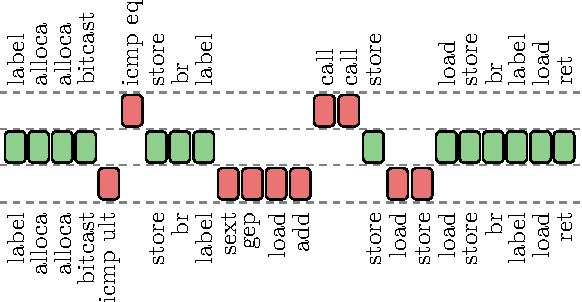
\includegraphics[width=0.75\linewidth]{figs/opcode-align.pdf}
  %\caption{An example of a sequence alignment between two real functions extracted from the \text{400.perlbench} benchmark.}
  \caption{The sequence alignment between two functions, identifying the equivalent segments of code (green in the center) and the non-equivalent ones (red at the sides).}
  \label{fig:opcode-align}
\end{figure}

Specifically for function-merging, we are concerned with the alphabet
consisting of all possible typed instructions and labels.
Every linearized function represents a sequence derived from this alphabet.
We explain the equivalence relation used for this alphabet in the next section.
Although we only consider pair-wise alignments, the technique would also work
for multi-sequences.

%We describe the equivalence relation between two predicated values in two
%separate cases, namely, the equivalence between instructions and the
%equivalence between labels.
%Labels are always considered equivalent.
%Two instructions are equivalent if their opcode are semantically equivalent,
%but not necessarily the same, and they both have types that can be bitcasted in
%a losslessly way from on to the other.
%This also includes making sure that there is no conflict regarding memory
%alignment when handling pointers.
%No additional restriction is imposed on the operands of the two instructions
%being compared for equivalence.
%Whenever two operands cannot be statically proved to represent the same value,
%a select instruction can be used to distinguish between the execution of two
%functions being merged.
%For function calls, the type equivalence requires that both instructions have
%identical function types, i.e., both called functions must have an identical
%return type and an identical list of parameter types.

%There is a vast literature on algorithms for performing sequence alignment,
%especially in the context of molecular biology.
%These algorithms range from optimal algorithms based on dynamic programming to
%probabilistic models that do not guarantee
%optimality~\cite{needleman70,smith81,carrillo88,hickey11}.
Our work uses the Needleman-Wunsch algorithm~\cite{needleman70} to perform sequence alignment.
This algorithm gives an alignment that is guaranteed to be optimal for a given scoring scheme~\cite{higgins89},
however, other algorithm could also be used with different performance and memory usage trade-offs~\cite{needleman70,smith81,carrillo88,hickey11}.
Different alignments would produce different but valid merged functions.

The Needleman-Wunsch algorithm~\cite{needleman70} is based on dynamic programming and consists of two main steps. First, it builds a \textit{similarity matrix}, based on a scoring scheme, which assigns weights
for matches, mismatches, and \textit{gaps} (blank characters). Afterwards, a backward traversal is performed on the similarity matrix, in
order to reconstruct the final alignment by maximizing the total score. We use a standard scoring scheme for the Needleman-Wunsch algorithm
that rewards matches and equally penalizes mismatches and gaps.

%\todo{Remove this paragraph.}
%When producing the final aligned sequence, there may be several possible optimal
%alignments.
%However, different aligned sequences can affect the code generation in different
%ways that may be both beneficial or undesirable.
%For this reason, we prioritize alignments that tend to group the blank
%characters together, avoiding to frequently alternate between the two sequences
%during long segments of mismatches and gaps.
%For example, note that in Figure~\ref{fig:opcode-align}, the red blocks, for
%a particular sequence, tend to be grouped together.


\subsection{Equivalence Evaluation}

Before we merge functions, we first need to define what makes two pieces of code equivalent and
therefore mergeable. In this section, we define equivalence in two separate cases, the equivalence
between instructions and the equivalence between labels.

In general, two instructions are equivalent if: $(1)$ their opcodes are semantically equivalent,
but not necessarily the same; $(2)$ they both have equivalent types; and $(3)$ they have pairwise
operands with equivalent types. Types are equivalent if they can be bitcast in a lossless way from one to
the other. For pointers, we also need to make sure that there is no conflict regarding memory alignment.
In the special case of function calls, type equivalence means that both instructions have identical
function types, i.e. identical return types and identical list of parameters.

Labels can represent both normal basic blocks and landing blocks used in exception handling code.
Labels of normal basic blocks are ignored during code equivalence evaluation, but we cannot do the
same for landing blocks. We describe how we handle such blocks in more detail in the following section.

\subsubsection{Exception Handling Code}

%%%%%%%%%%%%%%%%%%%%%%%%%%%%%%%%%%%%%%%%%%%%%%%
%%% RODRIGO: I think that we need to talk about landing blocks, not only landing pad instructions,
%%% because labels that represent landing blocks are treated differently from normal basic blocks,
%%% and this is essential handling this kind of code, which is the key for some of the huge reduction
%%% on the benchmarks 447.dealII, 482.omnetpp, etc.
%%%%%%%%%%%%%%%%%%%%%%%%%%%%%%%%%%%%%%%%%%%%%%%

Most modern compilers implement the zero-cost Itanium ABI for exception
handling~\cite{dinechin00}, including GCC and LLVM, sometimes called the
\textit{landing-pad} model.
%In this model, landing-pad instructions are used to encode which action is taken
%when an exception has been thrown.
This model consists of:
$(1)$ invoke instructions that have two successors, one for the normal execution and
one for handling exceptions, called the landing block;
$(2)$ landing-pad instructions that encode which action is taken when an exception has
been thrown.
The invoke instruction co-operates tightly with its landing block.
The landing block must have a landing-pad instruction as its first non-$\phi$
instruction.
As a result, two equivalent invoke instructions must also have landing blocks
with identical landing-pad instructions.
This verification is made easy by having the landing-pad instruction as the first
instruction in a landing block.
%This restriction can be easily checked since the landing-pad instruction is
%always the first instruction in a landing block. 
%Landing blocks are responsible for handling all catch clauses covering the
%particular call site, in the high-level code.
%All clauses are defined by the landing-pad instruction, which encodes the list of
%all exception and cleanup handlers.
Similarly, landing-pad instructions are equivalent if they have exactly the same
type and also encode identical lists of exception and cleanup handlers.
%\fixme{ZW: We need an example here.}
%% landingpad {i8*, 32}
%%     catch i8* null


%The return value of the landing-pad instruction is crucial in deciding what
%action to take when the landing block is entered, and corresponds to the return
%value of the personality function.

%In other words, when the unwinder executes the personality function (which
%is part of the language runtime), it stores its return value, and provides this return value in the result of the landing-pad
%instruction. Since the personality function has access to the part of the unwind tables generated from the landing-pad
%instruction, it can communicate information encoded in the unwind table to the landing block itself. In the libc++ runtime,
%the personality function returns a tuple consisting of a pointer to the exception object itself, and a “handler switch value”, an
%integer which corresponds to the index of a relevant “catch” clause of the landing-pad instruction, or a special value (−1)
%when no catch clauses match but a cleanup needs to be performed.

%The LLVM IR generated for the landing block then checks the handler switch value computed by the personality function,
%and transfers control to a cleanup or handler block accordingly.

%Finally, if the selected handler is a cleanup handler, the
%exception propagation (stack unwinding) needs to be resumed after the cleanup is done. This is achieved by the resume
%instruction, which expects as a parameter the same value that was returned by the corresponding landing-pad instruction
%which interrupted the exception propagation.
%Interestingly, there are no LLVM instructions for raising (throwing) exceptions. This is left entirely in the management
%of the language runtime, which needs to closely co-operate with the stack unwinding library anyway (the interface of the
%personality function is mandated by the stack unwinder).

\subsection{Code Generation}
The code generation phase is responsible for producing a new function from the output of the sequence alignment.
Our three main objectives are: merging the parameter lists; generating select instructions to choose the appropriate
operands in merged instructions; and constructing the CFG of the merged function.

Our approach can effectively handle multiple different function merging scenarios:
\begin{itemize}[noitemsep,topsep=3pt]
  \item identical functions,
  \item functions with differing bodies,
  \item functions with different parameter lists, 
  \item functions with different return types,
  \item and any combination of these cases.
\end{itemize}

%\subsubsection{Merged Parameters}

To maintain the semantics of the original functions, we must be able to pass their parameters to
the new merged function. The merged parameter list is the union of the original lists, with
placeholders of the correct type for any of the parameters. Maintaining the original order is not
important for maintaining semantics, so we make no effort to do so.
If the two functions have differing bodies, we add an extra binary parameter, called the function
identifier, to the merged list of parameters. This extra parameter is required for selecting code
that should be executed only for one of the merged functions.

Figure~\ref{fig:merged-params} depicts
how we merge the list of parameters of two functions.
First, we create the binary parameter that represents the function identifier,
one of the functions will be identified by the value \texttt{true} and the other
by the value \texttt{false}.
We then add all the parameters of one of the functions to the new list of
parameters.
Finally, for each parameter of the second function, we either reuse an existing
and available parameter of identical type from the first function or we add a
new parameter.
We keep track of the mapping between the lists of parameters of the
original functions and the merged function so that, later, we are able to
update the function calls.
When replacing the function calls to the new merged function, parameters that
are not used by the original function being called will receive undefined values.
%For this reason, it is important to be careful when merging the two functions
%in order to avoid creating unsafe computation on undefined values, which
%results in undefined behavior.

The reuse of parameters between the two merged functions provides the following
benefits:
%(1) it allows for a simpler function call, with fewer values to pass to the
%called function, reducing code size;
%(2) similarly, it reduces the frame of the merged function;
(1) it reduces the overheads associated with function call abstractions, such as,
reducing the number of values required to be communicated between functions.
(2) if both functions use merged parameters in similar ways, it will remove some
of the cases where we need select instructions to distinguish between the functions.

\begin{figure}[t!]
  \centering
  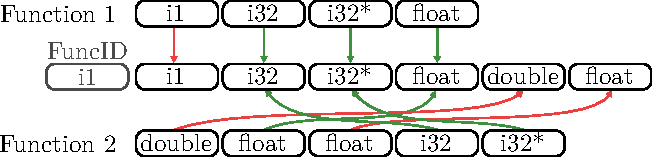
\includegraphics[width=0.9\linewidth]{figs/merged-params.pdf}
  \caption{Example of a merge operation on the parameter lists of two functions.}
  \label{fig:merged-params}
\end{figure}

There are multiple valid ways of merging parameter lists. For example, multiple
parameters of one function may have the same type as a given parameter from the other
function. In such cases, we select parameter pairs that minimize the number of
select instructions. We find them by analyzing all pairs of equivalent instruction
that use the parameters as operands. 
Our experiments show that maximizing the matching of parameters, compared to never
merging them, improves code-size reduction of individual benchmarks by up to 7\%.

%\subsubsection{Control-Flow Graph Reconstruction}

After generating the merged list of parameters, we produce the CFG of the merged function in two
passes over the aligned sequence.
The first pass creates the basic blocks and instructions.
The second assigns the correct operands to the instructions and connects the basic blocks.
A two-passes approach is required in order to handle loops, due to cyclic data dependencies.
%Listing~\ref{lst:CodeGen} presents the pseudocode for the code generation.

%\begin{myfloat}[h]
%  \begin{lstlisting}[caption={Pseudocode for the code generation. \todo{simplify.}}, label={lst:CodeGen}]
%CodeGen(Sequence, Function) {
% CFG = Function.NewCFG()
% VMap = Mapping of values to values
% MergedBB = null
% TailBB = Mapping of labels to labels
% //first pass: create CFG and instructions
% for each Entry in Sequence:
%   if Entry is a match:
%      if Entry is of labels:
%         BBLabel = CFG.NewBlock()
%         ValMap[Entry[0]] = BBLabel
%         ValMap[Entry[1]] = BBLabel
%         if Entry has landing-pad:
%           create landing-pad for BBLabel
%         MergedBB = BBLabel
%      if Entry is of instructions:
%         I0, I1 = Entry[0], Entry[1]
%         if MergedBB is null:
%           MergedBB = G.addBasicBlock()
%           TailBB[I0.getBlock()].addBranch(MergedBB)
%           TailBB[I1.getBlock()].addBranch(MergedBB)
%         add cloned instruction to MergedBB
%         if Entry is terminator instruction:
%           MergedBB = null
%   else:
%      if MergedBB not null:
%        branch to two new basic blocks
%        add new basic blocks to TailBB
%        MergedBB = null
%
%      if Entry is a label:
%        BBLabel = G.NewBlock()
%        ValMap[Entry] = BBLabel
%      if Entry is an instruction:
%        BB = TailBB[Entry.getBlock()]
%        add cloned instruction to the BB
%
% //second pass: update operands
% for each Entry in Sequence:
%   if Entry is a match:
%      if Entry is of instructions:
%         I0, I1 = Entry[0], Entry[1]
%         I = ValMap[I0]
%
%         for each (Op0, Op1) in I0 and I1:
%           Op0Val = ValMap[Op0]
%           Op1Val = ValMap[Op1]
%           OpVal = Op0Val //assuming equality
%           if ValMap[Op0]!=ValMap[Op1]:
%              OpVal = G.addSelect(Op0Val,Op1Val)
%           update operand of I with OpVal
%   else:
%      if Entry is an instruction:
%        I = ValMap[Entry]
%        update all operands of I using ValMap
%
%}
%  \end{lstlisting}
%\end{myfloat}

First, for each entry in the aligned sequence, we either create a new basic
block for labels or we add a cloned instruction to the appropriate basic
block.
If the label represents a landing block, a landing-pad instruction is also added
to the new basic block.
During this process, we keep a mapping from the instructions and labels in the
original functions to their corresponding values in the new merged function.
We need this mapping to generate the use-definition chains for the merged function, which is done by pointing the operands of the
instructions to the correct values in the function.
However, at this point, the cloned instructions are given empty operands,
as we are still creating the complete mapping.

While iterating over the aligned sequence, we also need to create extra basic
blocks and branch instructions in order to maintain the semantics of the
original functions, guarding the execution of instructions that are unique to
one of the functions being merged.
When transitioning from matching instructions or labels to non-matching ones,
we need to branch to new basic blocks based on the function identifier.
%This divergent point is used to continue code generation for the contiguous
%non-matching segment of the aligned sequence.
When transitioning back from non-matching segments to a matching segment, we need
to reconnect both divergent points by branching back to a single new basic block
where merged instructions will be added.
This process generates a diamond shaped structures in the CFG. %%TODO add figure


The second pass over the aligned sequence creates the operands of all the instructions.
%the operands of all the instructions and adds select instructions as necessary.
%Select instructions are created when a merged instruction has different operand
%values in the original functions, so the appropriate value needs to be
%selected based on the function identifier.
Operand mappings are performed as follows.
%We first map the instructions from the original functions to the corresponding ones in the merged function. Then, we use this mapping to create...
We use the previously created mapping in order to map the correct operands for each instruction in the merged function. The creation of operands can be divided in two main cases, non-matching and matching instructions. (1) Creating the operands for non-matching instructions (i.e. those that occur in just one function) is straightforward. In this case, we only need to use the value mapped by the original operand. (2) Matching instructions can have different values in corresponding operands in each one of the original functions. In this case, we need to use a select instruction to choose, at runtime, between these values. If the original operands map to different values $V_1$ and $V_2$, then we add a new select instruction ``select (func\_id==1), V\_1, V\_2", which computes the operand of the merged instruction. If these values are identical, we use this directly, without the need for a select.
%%TODO create a small figure with an example of the select instruction

If the operands are labels, instead of adding a select instruction, we perform
operand selection through divergent control flow, using a new basic
block and a conditional branch on the function identifier.
If the two labels represent landing blocks, we hoist the landing-pad
instruction to the new common basic block, converting it to a landing block and
converting the two landing blocks to normal basic blocks.
This is required for the correctness of the landing-pad model.
Similar to previous work on vectorization~\cite{porpodas18}, we
also exploit commutative instructions in order to maximize similarity.
When assigning operands to commutative instructions, we perform operand
reordering to maximize the number of matching operands and reduce the total
number of select instructions required.

It is important to note that if we are merging two identical functions, no
select or extra branch instruction will be added.
As a result, we can remove the extra parameter that represents the function
identifier.

%\vspace{-1ex}
\section{Focusing on Profitable Functions}
\label{sec:framework}

%In this section, we describe our implementation of the function merging
%optimization, which combines the proposed function-merging technique with an
%efficient exploration infrastructure.

%In this section, we describe our exploration infrastructure for the
%function merging optimization.
Although the proposed technique is able to merge any two functions, it is not always profitable to merge them. In fact, as it is only
profitable to merge functions that are sufficiently similar, for most pairs of functions, merging them increases code size.
In this section, we propose our framework for efficiently exploring the
optimization space, focusing on pairs of functions that are profitable to merge. 

%Therefore,
%the main goal of our exploration infrastructure is to efficiently find pairs of functions that are profitable to merge.
%%
%As described in Section~\ref{sec:background}, LLVM's existing function merging
%optimization, due to its hard restriction of only merging identical functions,
%is able to  efficiently explore which functions to merge by computing a hash
%of the functions.
%If two functions have the same hash, they are very likely to be identical.
%Moreover, merging identical functions is always profitable.
%For the proposed function-merging technique, on the other hand, because it is
%able to merge any pair of functions, we have a much larger exploration space and
%also a more challenging decision problem.

%\subsection{Ranking Infrastructure}

For every function, ideally, we would like to try to merge it with all other functions and choose the pair that maximizes the reduction in
code size. However, this quadratic exploration over all pairs of functions results in prohibitively expensive compilation
overhead. In order to avoid the quadratic exploration of all possible merges, we propose the exploration framework shown in
Figure~\ref{fig:func-merge-opt-arch} for our optimization.
\begin{figure}[t!]
  \centering
  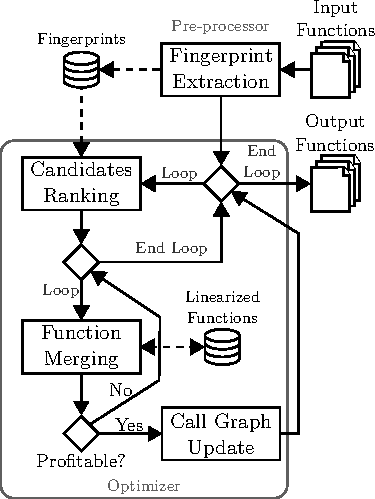
\includegraphics[width=0.65\linewidth]{figs/func-merge-opt-arch.pdf}
  \caption{Overview of our exploration framework.}
  \label{fig:func-merge-opt-arch}
\end{figure}

The proposed framework is based on a light-weight ranking infrastructure that uses a \textit{fingerprint} of the functions to evaluate
their similarity. It starts by first precomputing and caching the fingerprint of all functions. The goal of the fingerprint is to allow us
to efficiently discard unpromising pairs of functions so that we perform the more expensive evaluation only on the topmost similar pairs.
To this end, the fingerprint consists of: $(1)$ a map of instruction opcodes to their frequency in the function; $(2)$ the set of types
manipulated by the function. While functions can have several thousands of instructions, an IR usually has just a few tens of opcodes,
e.g., the LLVM IR has only about 64 different opcodes. This means that the fingerprint needs to store just a small integer array of the
opcode frequencies and a set of types, which allows for an efficient similarity comparison.

By comparing the opcode frequencies of two functions, we are able to estimate
an upper bound of the merge between these functions, assuming that all
instructions with the same opcode would always result in a match.
This assumption provides an upper bound on the actual number of matches, since
it may be affected by the instruction types and the order they appear in the
linearized functions.
As a way to refine this estimate, we weight this upper bound by the Jaccard
similarity coefficient~\cite{jaccard} of the sets of types, i.e., a
type-similarity ratio between the two functions.
Formally, let $T_1$ and $T_2$ be the set of types of the functions $f_1$ and
$f_2$, respectively.
Therefore, the upper-bound reduction, computed as a ratio, can be defined as
\vspace{-1.5ex}\[
   U\!B(f_1,f_2) = \frac{\sum\limits_{op \in Ops} \min\{freq(op,f_1),freq(op,f_2)\}}{\sum\limits_{op \in Ops} freq(op,f_1)+freq(op,f_2)}
\vspace{-1.5ex}
\]
and the weighted estimate is given by
\vspace{-1.5ex}\[
     s(f_1,f_2) = U\!B(f_1,f_2) \frac{|T_1 \cap T_2|}{|T_1 \cup T_2|}.
\vspace{-1.5ex}
\]
This weighted estimate results in a value in the range $[0,0.5]$,
which encodes a description that favors maximizing both the opcode and type
similarities, while also minimizing their respective differences.
Identical functions will always result in the maximum value of $0.5$.

For each function $f_1$, we use a priority queue to rank the topmost
similar candidates based on their similarity, defined by $s(f_1,f_2)$, for all
other functions $f_2$.
We use an exploration threshold to limit how many top candidates we will
evaluate for any given function.
This candidate exploration is then performed in a greedy fashion, where the first
candidate that actually results in a profitable merge ends the exploration and
the merge operation is finally committed.

\begin{figure}[t!]
  \centering
  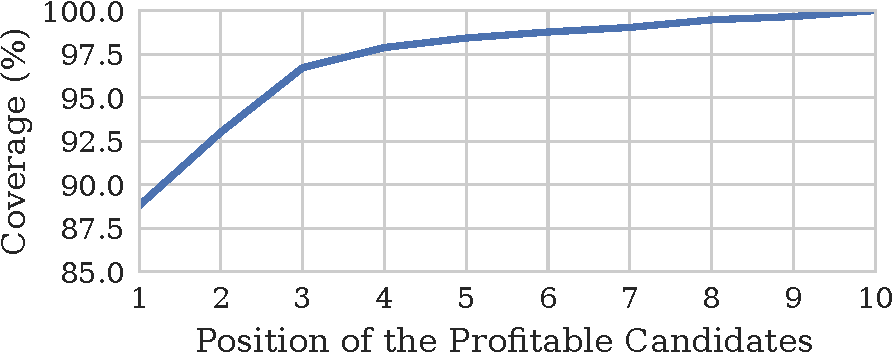
\includegraphics[width=0.8\linewidth]{figs/average-cdf-exploration-threshold.pdf}
  \caption{Average CDF for the exploration threshold and the percentage of merged operations covered.
           89\% of the merge operations happen with the topmost candidate.}
           %A merge operation happens with the topmost candidate in about 89\% of the cases.}
  \label{fig:average-cdf-exploration-threshold}
\end{figure}

Ideally, the profitable candidate will be as close to the top of the rank as
possible.
Figure~\ref{fig:average-cdf-exploration-threshold} shows the cumulative
distribution of the position of the profitable candidates in a top 10 rank.
It shows that about 89\% of the merge operations occurred with the topmost
candidate, while the top 5 cover over 98\% of the profitable candidates.
These results suggest that the proposed fingerprint similarity is able to
accurately capture the real function similarity, while reducing the exploration
cost by a few orders of magnitudes, depending on the actual number and size of
the functions.

When a profitable candidate is found, we first replace the body of the two
original functions to a single call to the merged function.
Afterwards, if the original functions can be completely removed, we update the
call graph, replacing the calls to the original functions by calls to the
merged function.
Finally, the new function is added to the optimization working list.
Because of this feedback loop, merge operations can also be performed on
functions that resulted from previous merge operations.

\subsection{Profitability Cost Model}\label{sec:profit-model}

After generating the code of the merged function, we need to estimate the
code-size benefit of replacing the original pair of functions by the new merged
function.
In order to estimate the code-size benefit, we first compute the code-size cost
for each instruction in all three functions.
In addition to measuring the difference in size of the merged function, we also
need to take into account all extra costs involved:
$(1)$ for the cases where we need to keep the original functions with a call to
the merged function;
and $(2)$ for the cases where we update the call graph, there might be an extra
cost with a call to the merged function due to the increased number of arguments.

Let $c(f)$ be the code-size cost of a given function $f$, and
$\delta(f_i, f_j)$ represent the extra costs involved when replacing or
updating function $f_i$ with the function $f_j$.
Therefore, given a pair of functions $\{f_1,f_2\}$ and the merged function
$f_{1,2}$, we want to maximize the profit defined as:
\[
  \Delta(\{f_1,f_2\},f_{1,2}) = (c(f_1)+c(f_2)) - (c(f_{1,2}) + \varepsilon)
\]
where $\varepsilon = \delta(f_1, f_{1,2}) + \delta(f_2, f_{1,2})$.
We consider that the merge operation is profitable if $\Delta(\{f_1,f_2\},f_{1,2})>0$.

However, because we are operating on the IR level, one IR instruction does not
necessarily translate to one machine instruction.
Because of that, the profitability is measured with the help of the compiler's
target-specific cost model.
The actual cost of each instruction comes from querying this compiler's built-in
cost model, which provides a target-dependent cost estimation that approximates
the code-size cost of an IR instruction when lowered to machine instructions.
Our implementation makes use of the code-size costs provided by LLVM's
target-transformation interface (TTI), which is widely used in the decision
%making by most of the LLVM's optimizations.
making of most optimizations.

\subsection{Link-Time Optimization}

There are different ways of applying this optimization, with different trade-offs.
We can apply our optimization on a per compilation-unit basis, which usually
results in lower compilation-time overheads, because only a small part of the
whole program is being considered at each moment.
However, this also limits the optimization opportunities, since only pairs of
functions within the same compilation unit would be merged.

On the other hand, our optimization can also be applied in the whole program,
for example, during link-time optimization (LTO).
Optimizing the whole program is beneficial for the simple fact that the
optimization will have more functions at its disposal.
It allows us to merge functions across modules.

In addition to the benefit of being able to merge more functions, when optimizing
the whole program, we can also be more aggressive when removing the original functions,
since we know that there will be no external reference to them.
However, if the optimization is applied per compilation unit, then extra
conditions must be guaranteed, e.g., the function must be explicitly defined
as internal or private to the compilation unit.

\begin{figure}[t!]
  \centering
  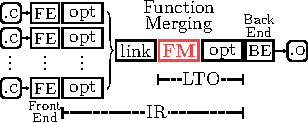
\includegraphics[width=0.7\linewidth]{figs/opt-pipeline.pdf}
  \caption{In our experiments we use a compilation pipeline with a monolithic link-time optimization (LTO).}
  \label{fig:opt-pipeline}
\end{figure}


Figure~\ref{fig:opt-pipeline} shows an overview of the compilation pipeline used
throughout our evaluation.
First, we apply early code-size optimizations to each compilation unit.
Then, function merging and further code-size optimizations are applied during
monolithic link-time optimization~(LTO).
With LTO, object file generation is delayed until all input modules are known,
instead of being generated per compilation unit, which enables more powerful
optimizations based on whole-program analyses.
